
\begin{exercise}

% 14 p. 88
 Twee duikers duiken horizontaal van een duikplatform. De bovenste duiker A start tweemaal hoger boven het water dan de onderste duiker. De horizontale beginsnelheid van de onderste duiker is tweemaal zo groot als die van de bovenste. De duikers komen terecht in het water op horizontale afstanden $x_a$ en $x_b$ van de plank. Wat is de verhouding van de horizontale afstanden?
%\newline
%\newline
%\begin{tabularx}{\textwidth}{XXXX}
%(a) $\displaystyle\frac{x_a}{x_b}=\frac{1}{\sqrt{2}}$&(b) $\displaystyle\frac{x_a}{x_b}=1$&(c) $\displaystyle\frac{x_a}{x_b}=\sqrt{2}$&(d) $\displaystyle\frac{x_a}{x_b}=2$
%\end{tabularx}
%
%\begin{figure}[H]
%\centering
%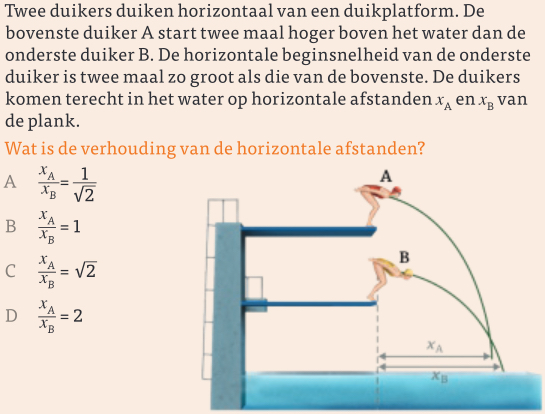
\includegraphics[width=0.6\textwidth]{dyn/exercises/14p88}
%\end{figure}
\begin{minipage}[t]{.3\textwidth}
\begin{enumerate}
\item $\displaystyle\frac{x_a}{x_b}=\frac{1}{\sqrt{2}}$
\item $\displaystyle\frac{x_a}{x_b}=1$
\item $\displaystyle\frac{x_a}{x_b}=\sqrt{2}$
\item $\displaystyle\frac{x_a}{x_b}=2$
\end{enumerate}
\end{minipage}
\hfill
\begin{minipage}[t]{.5\textwidth}
	\raisebox{1ex-\height}{%
		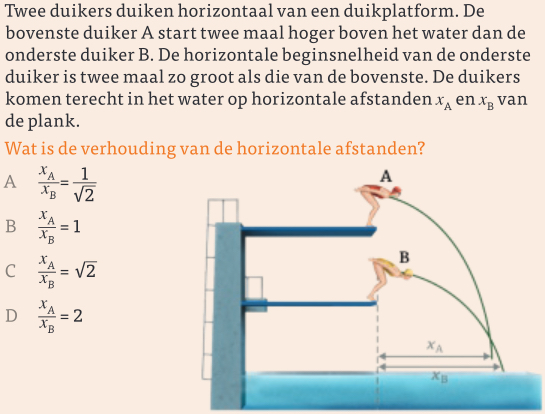
\includegraphics[width=\textwidth]{dyn/exercises/14p88}} 
\end{minipage}
\begin{oplossing}
% \newline
In verticale zin hebben beide duikers geen beginsnelheid en versnellen ze met de valversnelling. In verticale zin voeren ze dus een EVRB uit. De valtijd vind je dan uit $y=\frac{1}{2}gt^2$, nl. $t=\sqrt{\frac{2y}{g}}$.

In horizontale zin hebben de duikers geen versnelling en houden dus (volgens de wet van de traagheid) hun initi\"ele snelheid aan. De afgelegde weg volgens de horizontale $x$-as vinden we dan ook met $x=v_0t$ waarin $v_0$ de (horizontale) beginsnelheid is en waarin we $t$ door de valtijd kunnen vervangen.

Gebruik nu dat $y_a=2y_b$ en $v_{0b}=2v_{0a}$ en bereken de gevraagde verhouding.
\end{oplossing}

\end{exercise}
